% SMA-1 Graphical abstract.
% Generalist LLM (fluent, unreliable on the rare tail) + SMA memory
% (structure-mapping over a curated ontology) -> reliable, attributable
% specialist that cites, abstains, flags novelty. Iconographic, <= 1 column.
% Conceptual only. NO metrics. Caption supplied by manuscript.
\documentclass[border=4pt]{standalone}
\usepackage{amsmath}
\usepackage{amssymb}
\usepackage{pifont}
\usepackage{fontspec}
\setsansfont{Arimo}
\renewcommand{\familydefault}{\sfdefault}
\usepackage{tikz}
\usetikzlibrary{arrows.meta,positioning,calc,fit,backgrounds,shapes.geometric,decorations.pathmorphing}

\definecolor{ink}{HTML}{1A1C1E}
\definecolor{ink7}{HTML}{3D4248}
\definecolor{ink5}{HTML}{6B7177}
\definecolor{ink4}{HTML}{8A9097}
\definecolor{ink3}{HTML}{B4B9BE}
\definecolor{ink2}{HTML}{D6D9DC}
\definecolor{ink1}{HTML}{EAECEE}
\definecolor{ink05}{HTML}{F4F5F6}
\definecolor{teal}{HTML}{3F8A83}
\definecolor{teal2}{HTML}{4FA89F}
\definecolor{tealtint}{HTML}{E6F0EF}
\definecolor{amber}{HTML}{C2883C}
\definecolor{ambertint}{HTML}{F6ECDD}
\definecolor{redf}{HTML}{C05A50}
\definecolor{redtint}{HTML}{F6E2E0}
\definecolor{greenk}{HTML}{3E9B63}
\definecolor{greentint}{HTML}{E2F0E8}
\definecolor{fo}{HTML}{5AA9C4}
\definecolor{ho}{HTML}{2E6B86}
\definecolor{vio}{HTML}{9B86C4}
\definecolor{viotint}{HTML}{ECE6F4}

\newcommand{\BL}{\bfseries\fontsize{8}{9.5}\selectfont}
\newcommand{\NL}{\mdseries\fontsize{6.4}{7.6}\selectfont}

\begin{document}
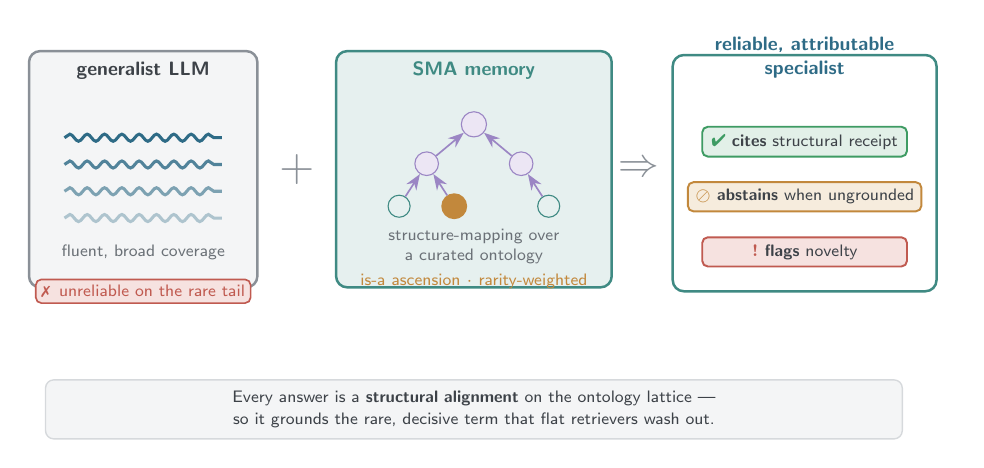
\begin{tikzpicture}[
  font=\sffamily,
  >=Stealth,
  hcap/.style={font=\sffamily\bfseries\fontsize{7.4}{8.6}\selectfont, text=ink7, align=center},
  sub/.style={font=\sffamily\fontsize{6.2}{7.4}\selectfont, text=ink5, align=center},
  tiny/.style={font=\sffamily\fontsize{5.6}{6.6}\selectfont, text=ink5, align=center},
  plus/.style={font=\sffamily\bfseries\fontsize{16}{16}\selectfont, text=ink4},
  bigarr/.style={-{Stealth[length=4mm,width=3.2mm]}, line width=1.6pt, color=teal2},
  card/.style={draw, line width=0.9pt, rounded corners=4pt, align=center, inner sep=4pt},
]

% ===================================================================
% Single panel, ~ 11.5 wide x 7.6 tall (column-friendly aspect).
% LLM  (+)  SMA memory  (=>)  attributable specialist {cite,abstain,novelty}
% ===================================================================

% ---------------- LEFT: generalist LLM ----------------
\node[card, draw=ink4, fill=ink05, minimum width=2.9cm, minimum height=3.0cm] (llm) at (1.75,4.6) {};
\node[hcap, text=ink7] at (1.75,5.85) {generalist LLM};
% "brain / fluent" glyph: wavy speech lines (fluent) with a faded tail
\foreach \i/\w in {0/1.0,1/0.82,2/0.6,3/0.35} {
  \draw[line width=1.1pt, color=ho, opacity=\w, decorate, decoration={snake, amplitude=0.45mm, segment length=2.2mm}]
        (0.75,5.0-0.34*\i) -- (2.75,5.0-0.34*\i);
}
\node[sub, text width=2.7cm] at (1.75,3.55) {fluent, broad coverage};
% rare-tail failure chip
\node[draw=redf, fill=redtint, rounded corners=2pt, line width=0.6pt, text=redf,
      font=\sffamily\fontsize{5.6}{6.6}\selectfont, inner sep=2pt] at (1.75,3.05)
      {\ding{55}\, unreliable on the rare tail};

% plus
\node[plus] at (3.7,4.6) {$+$};

% ---------------- MIDDLE: SMA memory ----------------
\node[card, draw=teal, fill=tealtint, minimum width=3.5cm, minimum height=3.0cm] (sma) at (5.95,4.6) {};
\node[hcap, text=teal] at (5.95,5.85) {SMA memory};
% mini is-a lattice + functor overlay glyph
\begin{scope}[shift={(5.95,4.55)}]
  % lattice
  \node[circle, draw=vio, fill=viotint, minimum size=3.2mm, inner sep=0pt] (r) at (0,0.62) {};
  \node[circle, draw=vio, fill=viotint, minimum size=3.0mm, inner sep=0pt] (m1) at (-0.6,0.12) {};
  \node[circle, draw=vio, fill=viotint, minimum size=3.0mm, inner sep=0pt] (m2) at (0.6,0.12) {};
  \node[circle, draw=teal, fill=tealtint, minimum size=2.8mm, inner sep=0pt] (l1) at (-0.95,-0.42) {};
  % lit rare node
  \node[circle, draw=amber, fill=amber, line width=0.8pt, minimum size=3.0mm, inner sep=0pt] (l2) at (-0.25,-0.42) {};
  \begin{scope}[on background layer]\node[circle, draw=amber!55, minimum size=5mm] at (-0.25,-0.42) {};\end{scope}
  \node[circle, draw=teal, fill=tealtint, minimum size=2.8mm, inner sep=0pt] (l3) at (0.95,-0.42) {};
  \draw[->, line width=0.6pt, color=vio] (m1)--(r); \draw[->, line width=0.6pt, color=vio] (m2)--(r);
  \draw[->, line width=0.6pt, color=vio] (l1)--(m1); \draw[->, line width=0.6pt, color=vio] (l2)--(m1); \draw[->, line width=0.6pt, color=vio] (l3)--(m2);
\end{scope}
\node[sub, text width=3.3cm] at (5.95,3.62) {structure-mapping over\\a curated ontology};
\node[tiny, text=amber] at (5.95,3.18) {is-a ascension $\cdot$ rarity-weighted};

% combine arrow
\node[plus, scale=0.85] at (8.05,4.6) {$\Rightarrow$};

% ---------------- RIGHT: attributable specialist ----------------
\node[card, draw=teal, fill=white, minimum width=3.35cm, minimum height=3.0cm] (spec) at (10.15,4.55) {};
\node[hcap, text=ho, text width=3.6cm] at (10.15,6.02) {reliable, attributable\\specialist};
% the three capabilities as stacked iconographic chips
\node[draw=greenk, fill=greentint, rounded corners=2pt, line width=0.7pt, text=ink7,
      font=\sffamily\fontsize{6.2}{7.2}\selectfont, minimum width=2.6cm, align=left, inner sep=2.6pt] (cci) at (10.15,4.95)
      {\textbf{\textcolor{greenk}{\ding{52}} cites} structural receipt};
\node[draw=amber, fill=ambertint, rounded corners=2pt, line width=0.7pt, text=ink7,
      font=\sffamily\fontsize{6.2}{7.2}\selectfont, minimum width=2.6cm, align=left, inner sep=2.6pt] (cab) at (10.15,4.25)
      {\textbf{\textcolor{amber}{$\oslash$} abstains} when ungrounded};
\node[draw=redf, fill=redtint, rounded corners=2pt, line width=0.7pt, text=ink7,
      font=\sffamily\fontsize{6.2}{7.2}\selectfont, minimum width=2.6cm, align=left, inner sep=2.6pt] (cnv) at (10.15,3.55)
      {\textbf{\textcolor{redf}{$\boldsymbol{!}$} flags} novelty};

% bottom one-line mechanism strip (qualitative, no metrics)
\node[draw=ink2, fill=ink05, rounded corners=3pt, line width=0.5pt, text=ink7,
      font=\sffamily\fontsize{6.4}{8}\selectfont, align=center, inner sep=4pt, text width=10.6cm] (strip) at (5.95,1.55)
      {Every answer is a \textbf{structural alignment} on the ontology lattice ---\\so it grounds the rare, decisive term that flat retrievers wash out.};

\end{tikzpicture}
\end{document}
